\documentclass{article}

\usepackage{geometry}
\usepackage{amsmath}
\usepackage{graphicx, eso-pic}
\usepackage{listings}
\usepackage{hyperref}
\usepackage{multicol}
\usepackage{fancyhdr}
\pagestyle{fancy}
\fancyhf{}
\hypersetup{ colorlinks=true, linkcolor=black, filecolor=magenta, urlcolor=cyan}
\geometry{ a4paper, total={170mm,257mm}, top=40mm, right=20mm, bottom=20mm, left=20mm}
\setlength{\parindent}{0pt}
\setlength{\parskip}{0.3em}
\renewcommand{\headrulewidth}{0pt}
\AddToShipoutPictureBG{%
  \AtPageUpperLeft{%
    \raisebox{-\height}{
\includegraphics[width=\paperwidth, height=30mm]{../headerarkav.png}}
  }
}
\rfoot{\thepage}
\lfoot{Final Competitive Programming - Arkavidia 7.0}
\lstset{
    basicstyle=\ttfamily\small,
    columns=fixed,
    extendedchars=true,
    breaklines=true,
    tabsize=2,
    prebreak=\raisebox{0ex}[0ex][0ex]{\ensuremath{\hookleftarrow}},
    frame=none,
    showtabs=false,
    showspaces=false,
    showstringspaces=false,
    prebreak={},
    keywordstyle=\color[rgb]{0.627,0.126,0.941},
    commentstyle=\color[rgb]{0.133,0.545,0.133},
    stringstyle=\color[rgb]{01,0,0},
    captionpos=t,
    escapeinside={(\%}{\%)}
}

\begin{document}

\begin{center}
    \section*{H - Hiasan Dinding} % ganti judul soal

    \begin{tabular}{ | c c | }
        \hline
        Batas Waktu  & 1s \\    % jangan lupa ganti time limit
        Batas Memori & 128MB \\  % jangan lupa ganti memory limit
        \hline
    \end{tabular}
\end{center}

\subsection*{Deskripsi}

Arvy telah menghias dinding raksasanya. Dinding raksasa Arvy dapat digambarkan sebagai bidang kartesius yang membentang menuju tak hingga ke arah sumbu-$x$ dan sumbu-$y$ (positif dan negatif). Hiasan dinding Arvy berupa $N$ buah paku tipis yang menancap di dinding. Paku-paku tersebut memiliki \textbf{koordinat bilangan bulat} dan membentuk \textbf{poligon konveks}.

Arvy akan bermain-main dengan hiasan dindingnya selama $Q$ hari. Pada awal setiap hari, Arvy akan memilih sepasang bilangan bulat $L$ dan $R$ dan melepas paku-paku tertentu dari dindingnya. Paku pada koordinat $(X_P,Y_P)$ akan dilepas apabila memenuhi salah satu dari dua syarat $X_P < L$ atau $X_P > R$. Lalu, Arvy akan memasang karet gelang raksasa pada dindingnya sehingga karet gelang tersebut membentuk \textbf{poligon konveks terkecil} yang memuat seluruh paku yang ada di dinding. Sebelum hari berikutnya, Arvy akan melepas karet gelang raksasanya dan memasang kembali paku-paku yang dilepasnya.

Dapatkah Anda mencari luas poligon yang dibentuk karet gelang Arvy setiap hari?

\textbf{Catatan:} 
\begin{itemize}
    \setlength\itemsep{0pt}
    \item{Poligon disebut konveks apabila setiap garis yang menyinggung sisinya tidak melewati bagian dalam poligon.}
    \item{Poligon yang memiliki kurang dari tiga titik sudut dianggap memiliki luas nol.}
    \item{Poligon yang seluruh titik sudutnya berada pada garis yang sama dianggap memiliki luas nol.}
\end{itemize}

\subsection*{Format Masukan}
Baris pertama berisi sebuah bilangan bulat $N$ $(3 \leq N \leq 2 \times 10^{5})$ yang menyatakan banyak paku di dinding Arvy.

$N$ baris berikutnya berisi sepasang bilangan bulat $X_i$ dan $Y_i$ $(-10^{9} \leq X_i,Y_i \leq 10^{9})$ yang menyatakan koordinat paku di dinding Arvy. Koordinat-koordinat paku membentuk poligon konveks dan diurutkan searah jarum jam dimulai dari paku yang berada di kiri-bawah (yang memiliki absis $(X_i)$ terkecil dan memiliki ordinat $(Y_i)$ terkecil). Tidak ada dua paku yang memiliki koordinat yang sama. Mungkin terdapat lebih dari dua paku yang terletak pada garis yang sama.

Baris berikutnya berisi sebuah bilangan bulat $Q$ $(1 \leq Q \leq 2 \times 10^{5})$ yang menyatakan banyaknya hari.

$Q$ baris berikutnya berisi sepasang bilangan bulat $L_i$ dan $R_i$ $(-10^{9} \leq L_i \leq R_i \leq 10^{9})$ yang menyatakan pasangan bilangan yang dipilih Arvy.

\subsection*{Format Keluaran}
$Q$ baris berisi sebuah bilangan riil dengan \textbf{satu angka di belakang titik} yang menyatakan luas poligon yang dibentuk karet gelang Arvy.

\pagebreak

\begin{multicols}{2}
\subsection*{Contoh Masukan}
\begin{lstlisting}
9
0 -1
0 0
1 1
3 2
5 1
6 0
5 -2
3 -3
1 -2
6
0 6
1 5
0 3
5 6
7 9
4 4

\end{lstlisting}
\columnbreak
\subsection*{Contoh Keluaran}
\begin{lstlisting}
19.5
16.0
10.0
1.5
0.0
0.0
\end{lstlisting}
\vfill
\null
\end{multicols}

\subsection*{Penjelasan}
Hiasan dinding Arvy berbentuk seperti berikut.
\begin{center}
\fbox{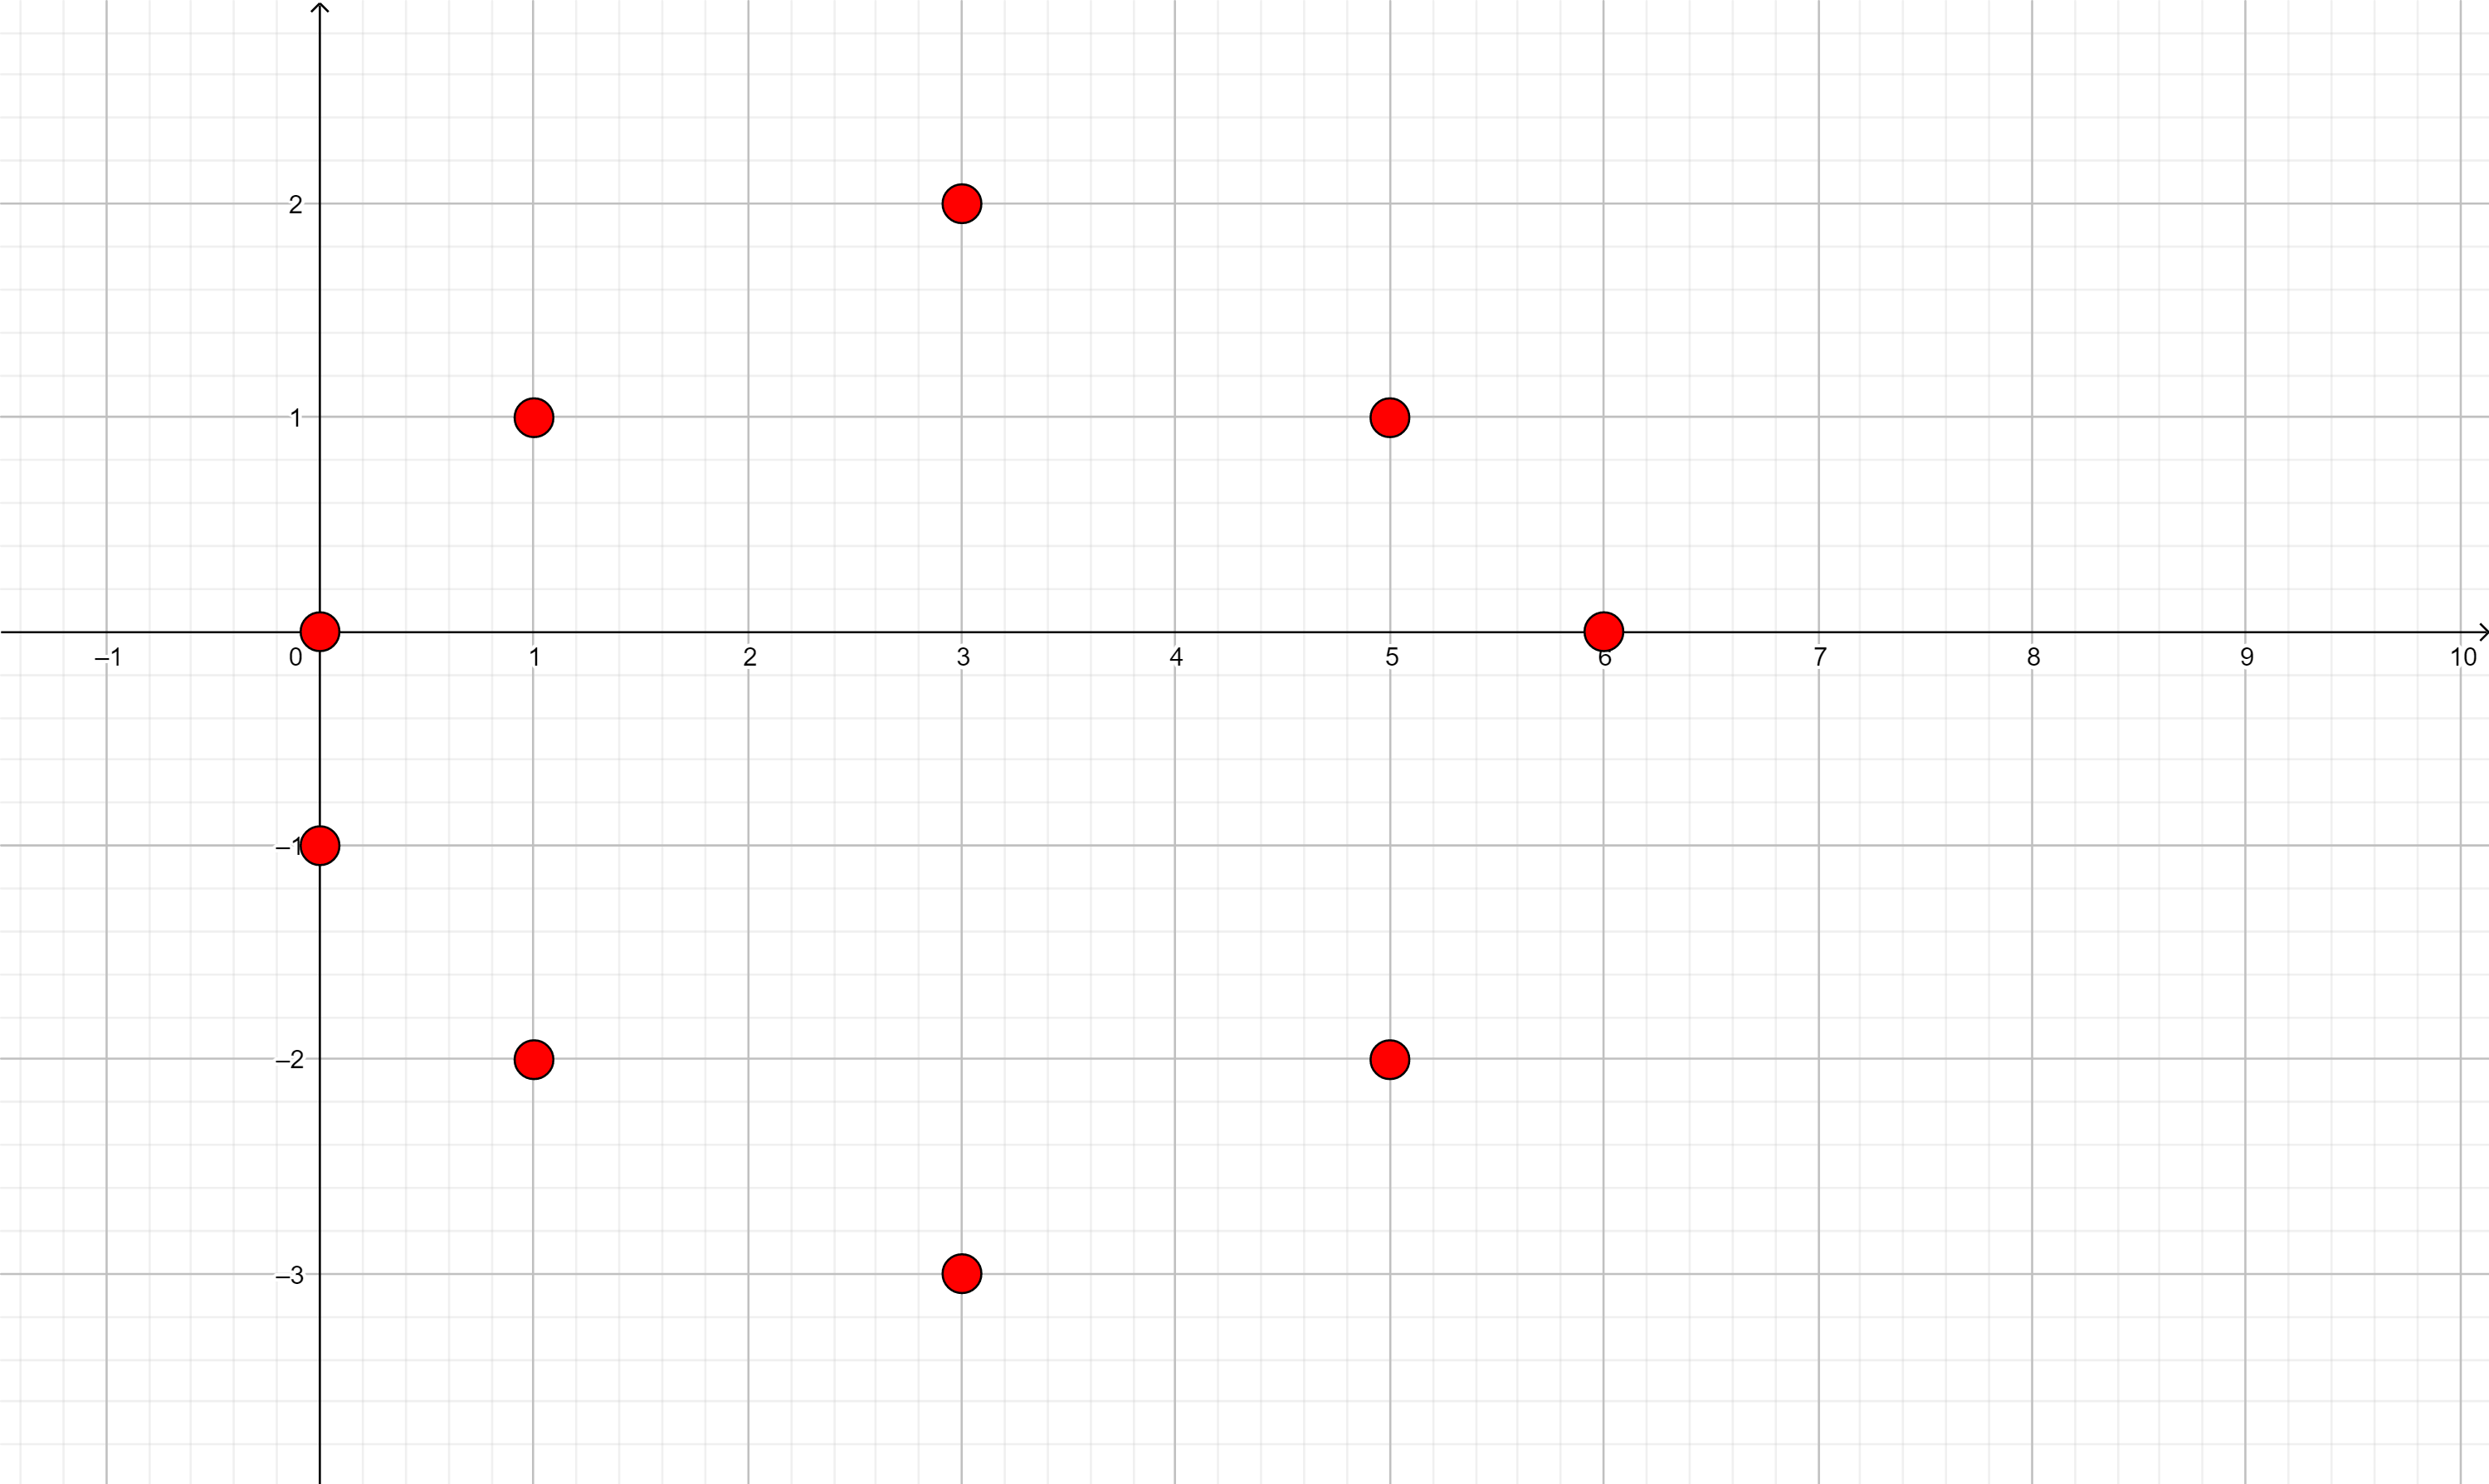
\includegraphics[scale=0.5]{points.png}}
\end{center}
Poligon yang dibentuk karet gelang Arvy pada hari ke-1 sampai ke-4 berbentuk seperti berikut.
\begin{center}
\fbox{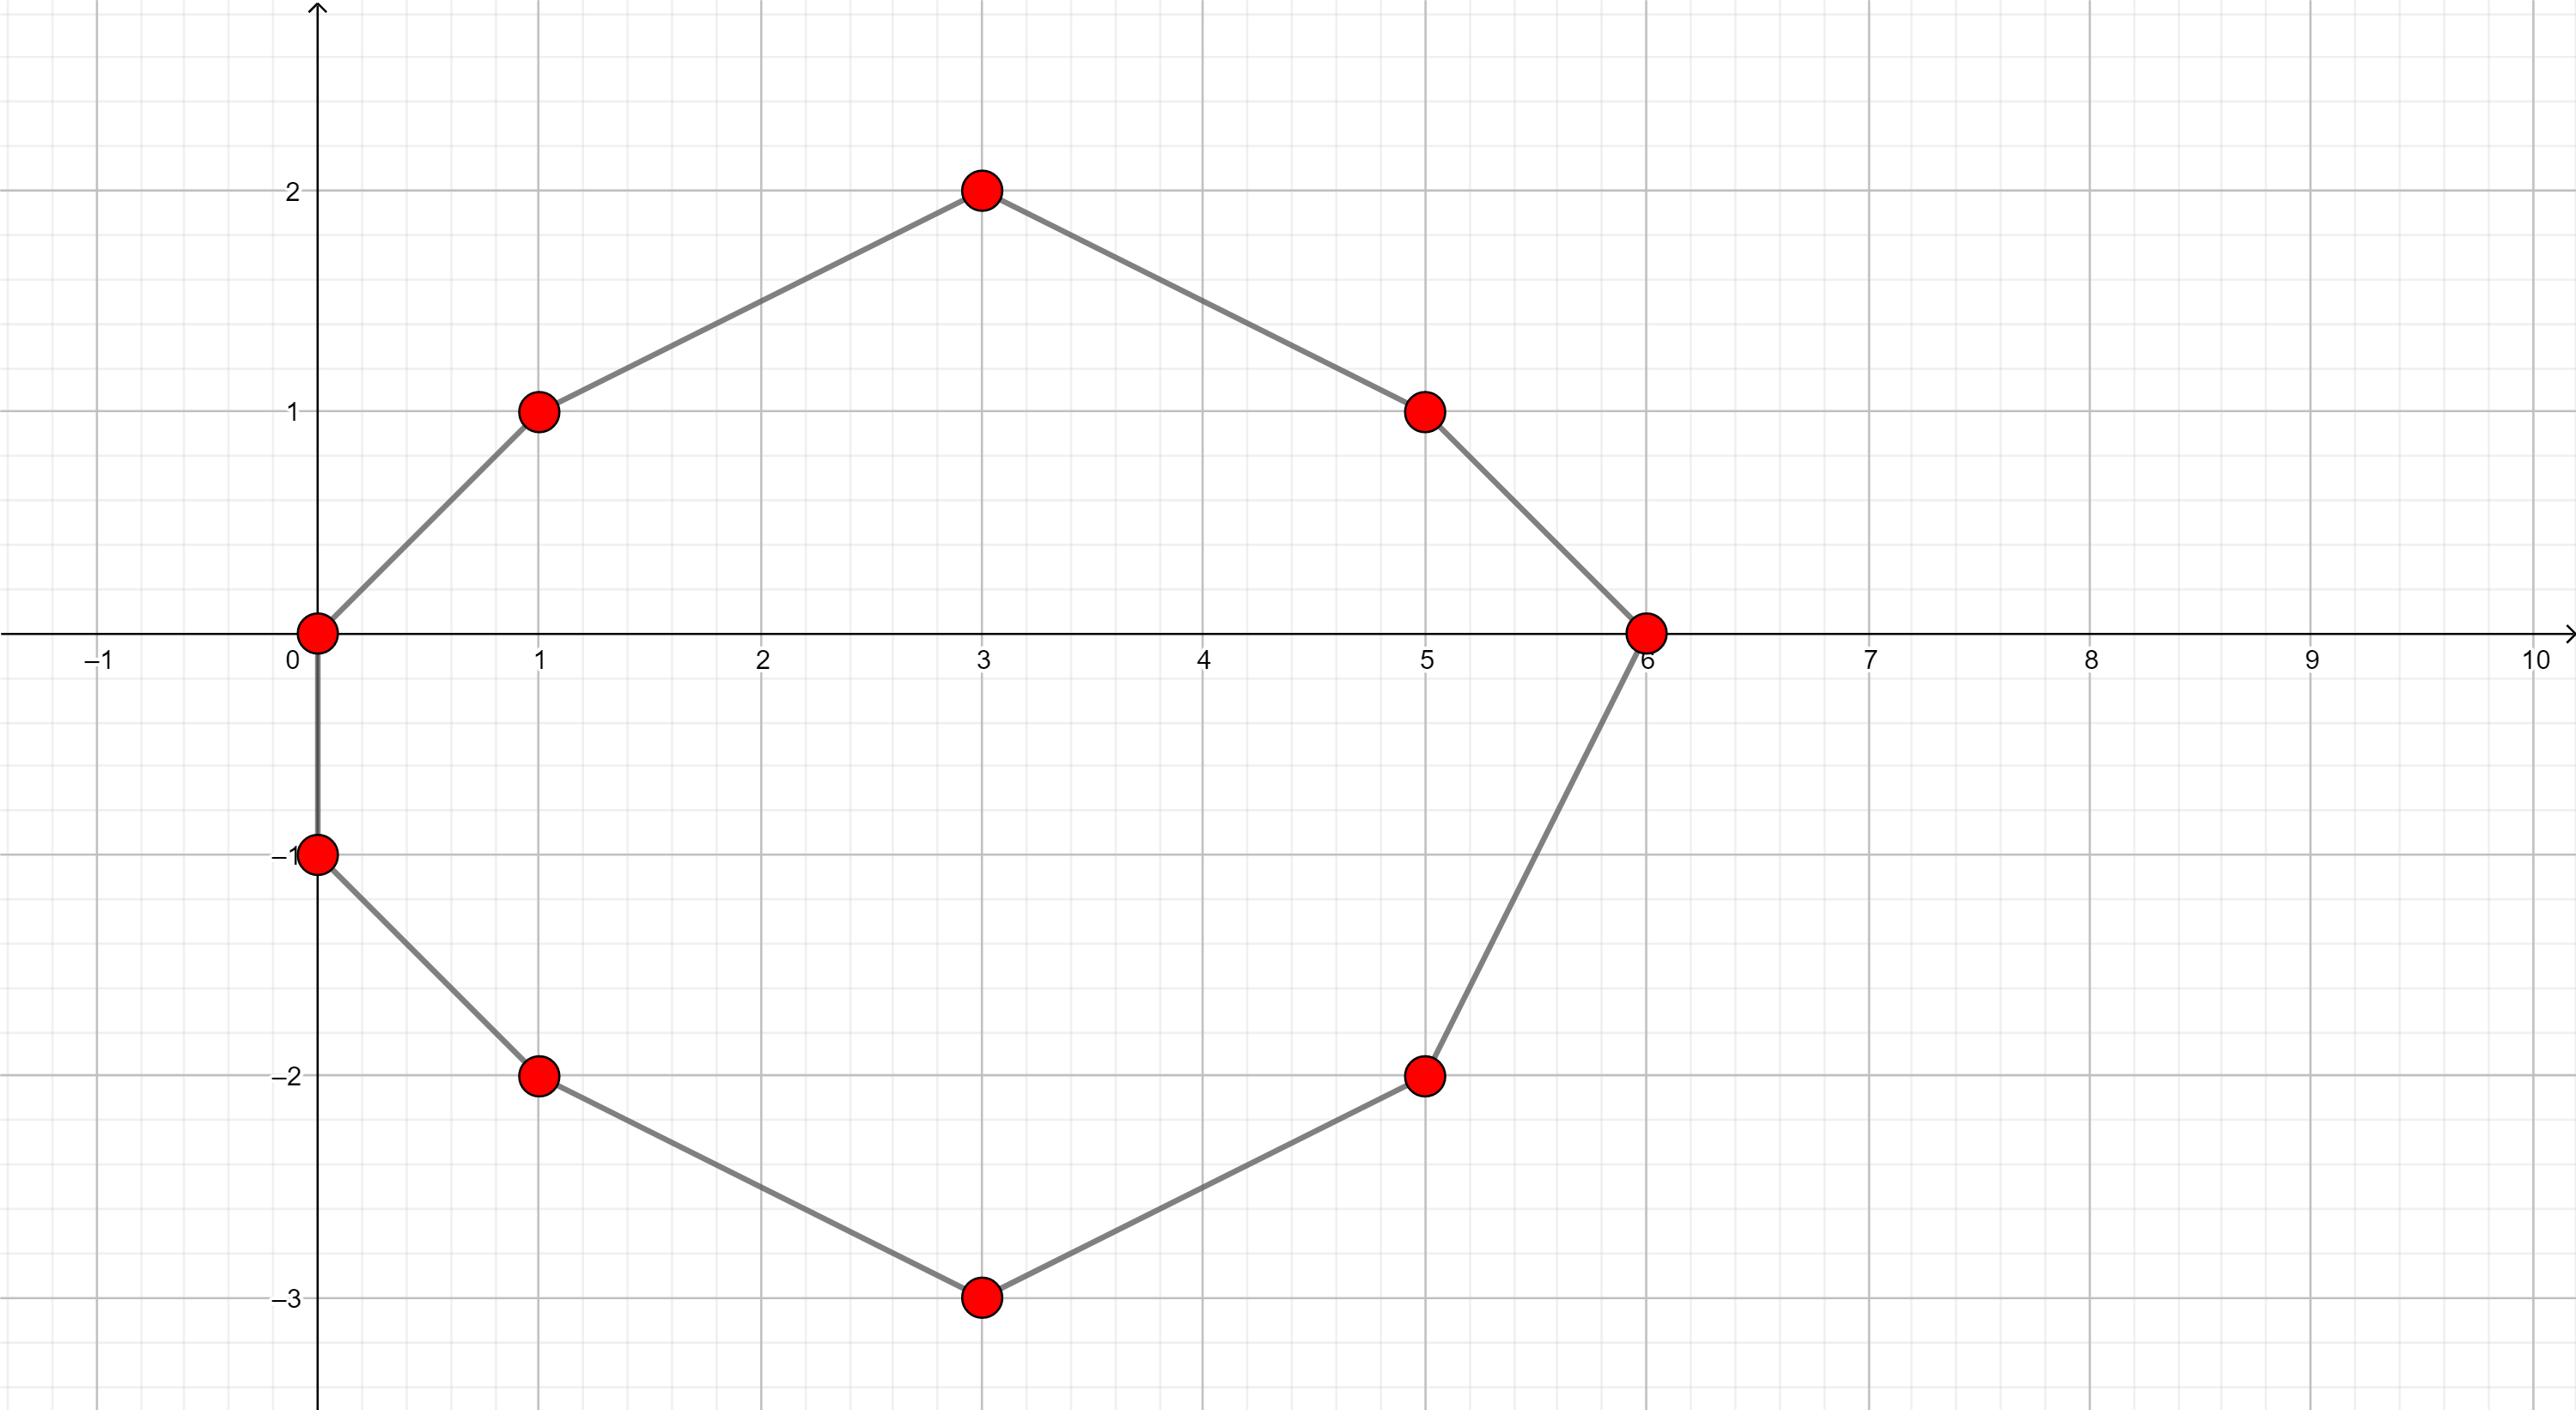
\includegraphics[scale=0.5]{poly1.png}}
\fbox{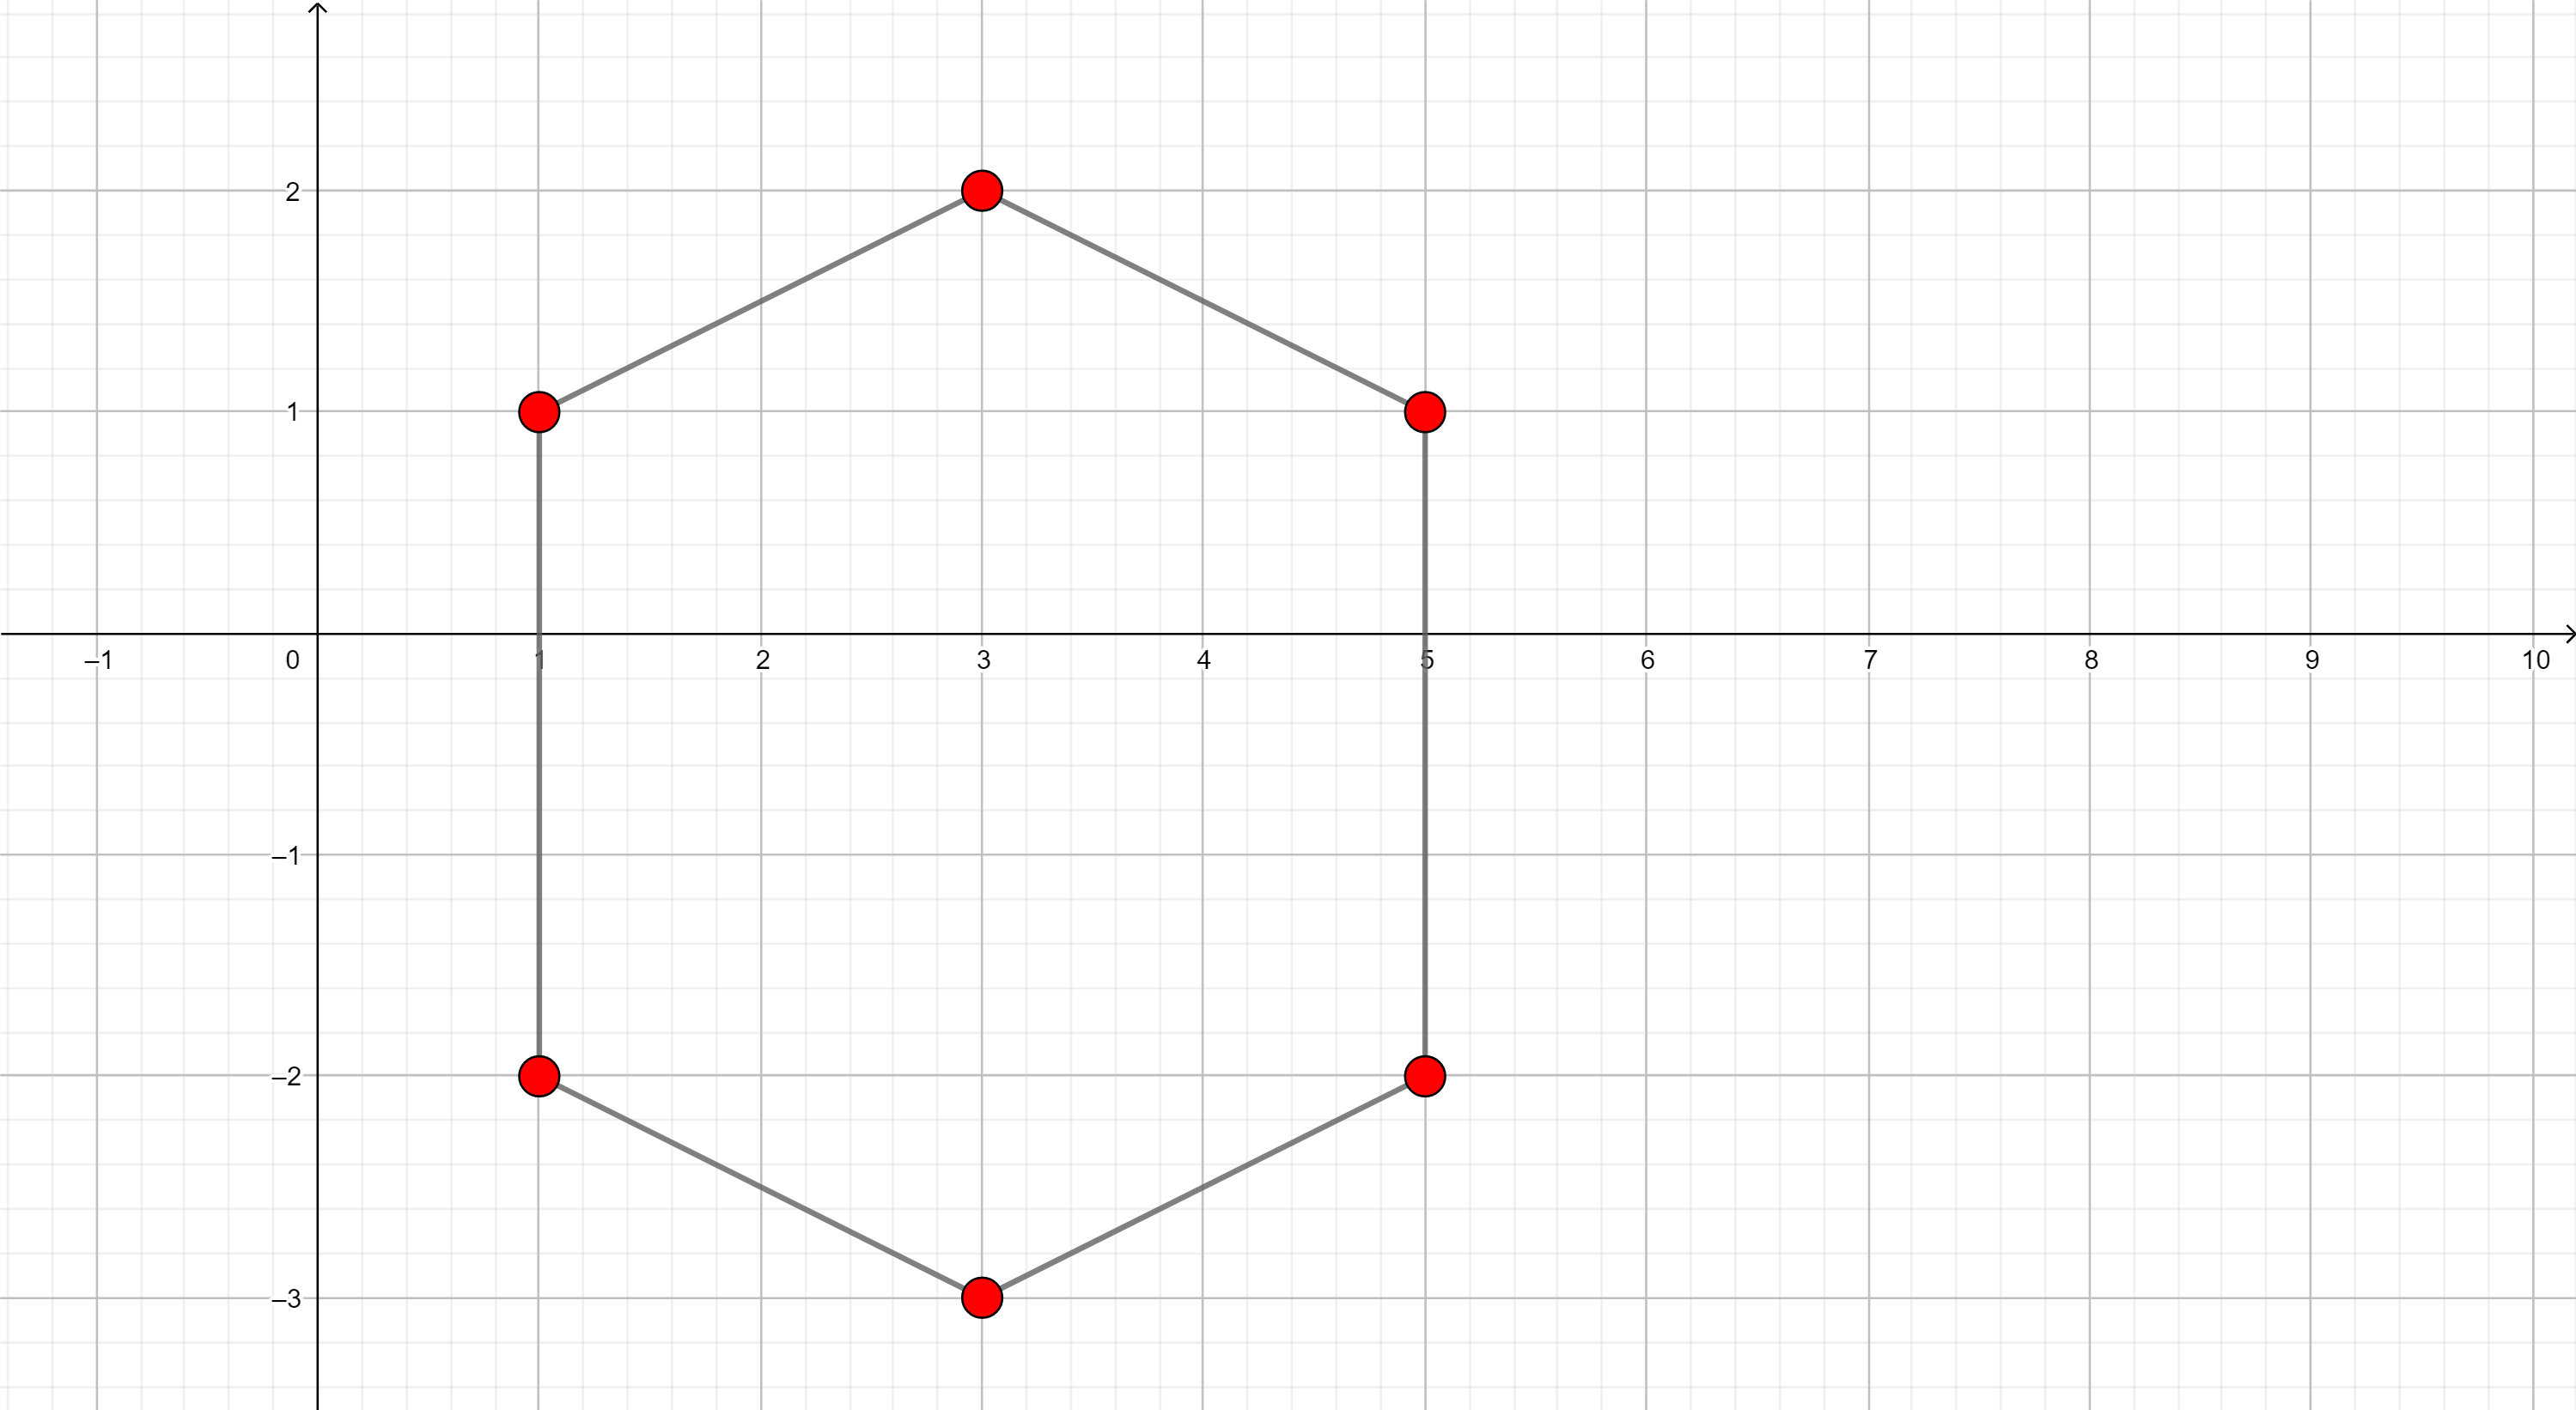
\includegraphics[scale=0.5]{poly2.png}}
\fbox{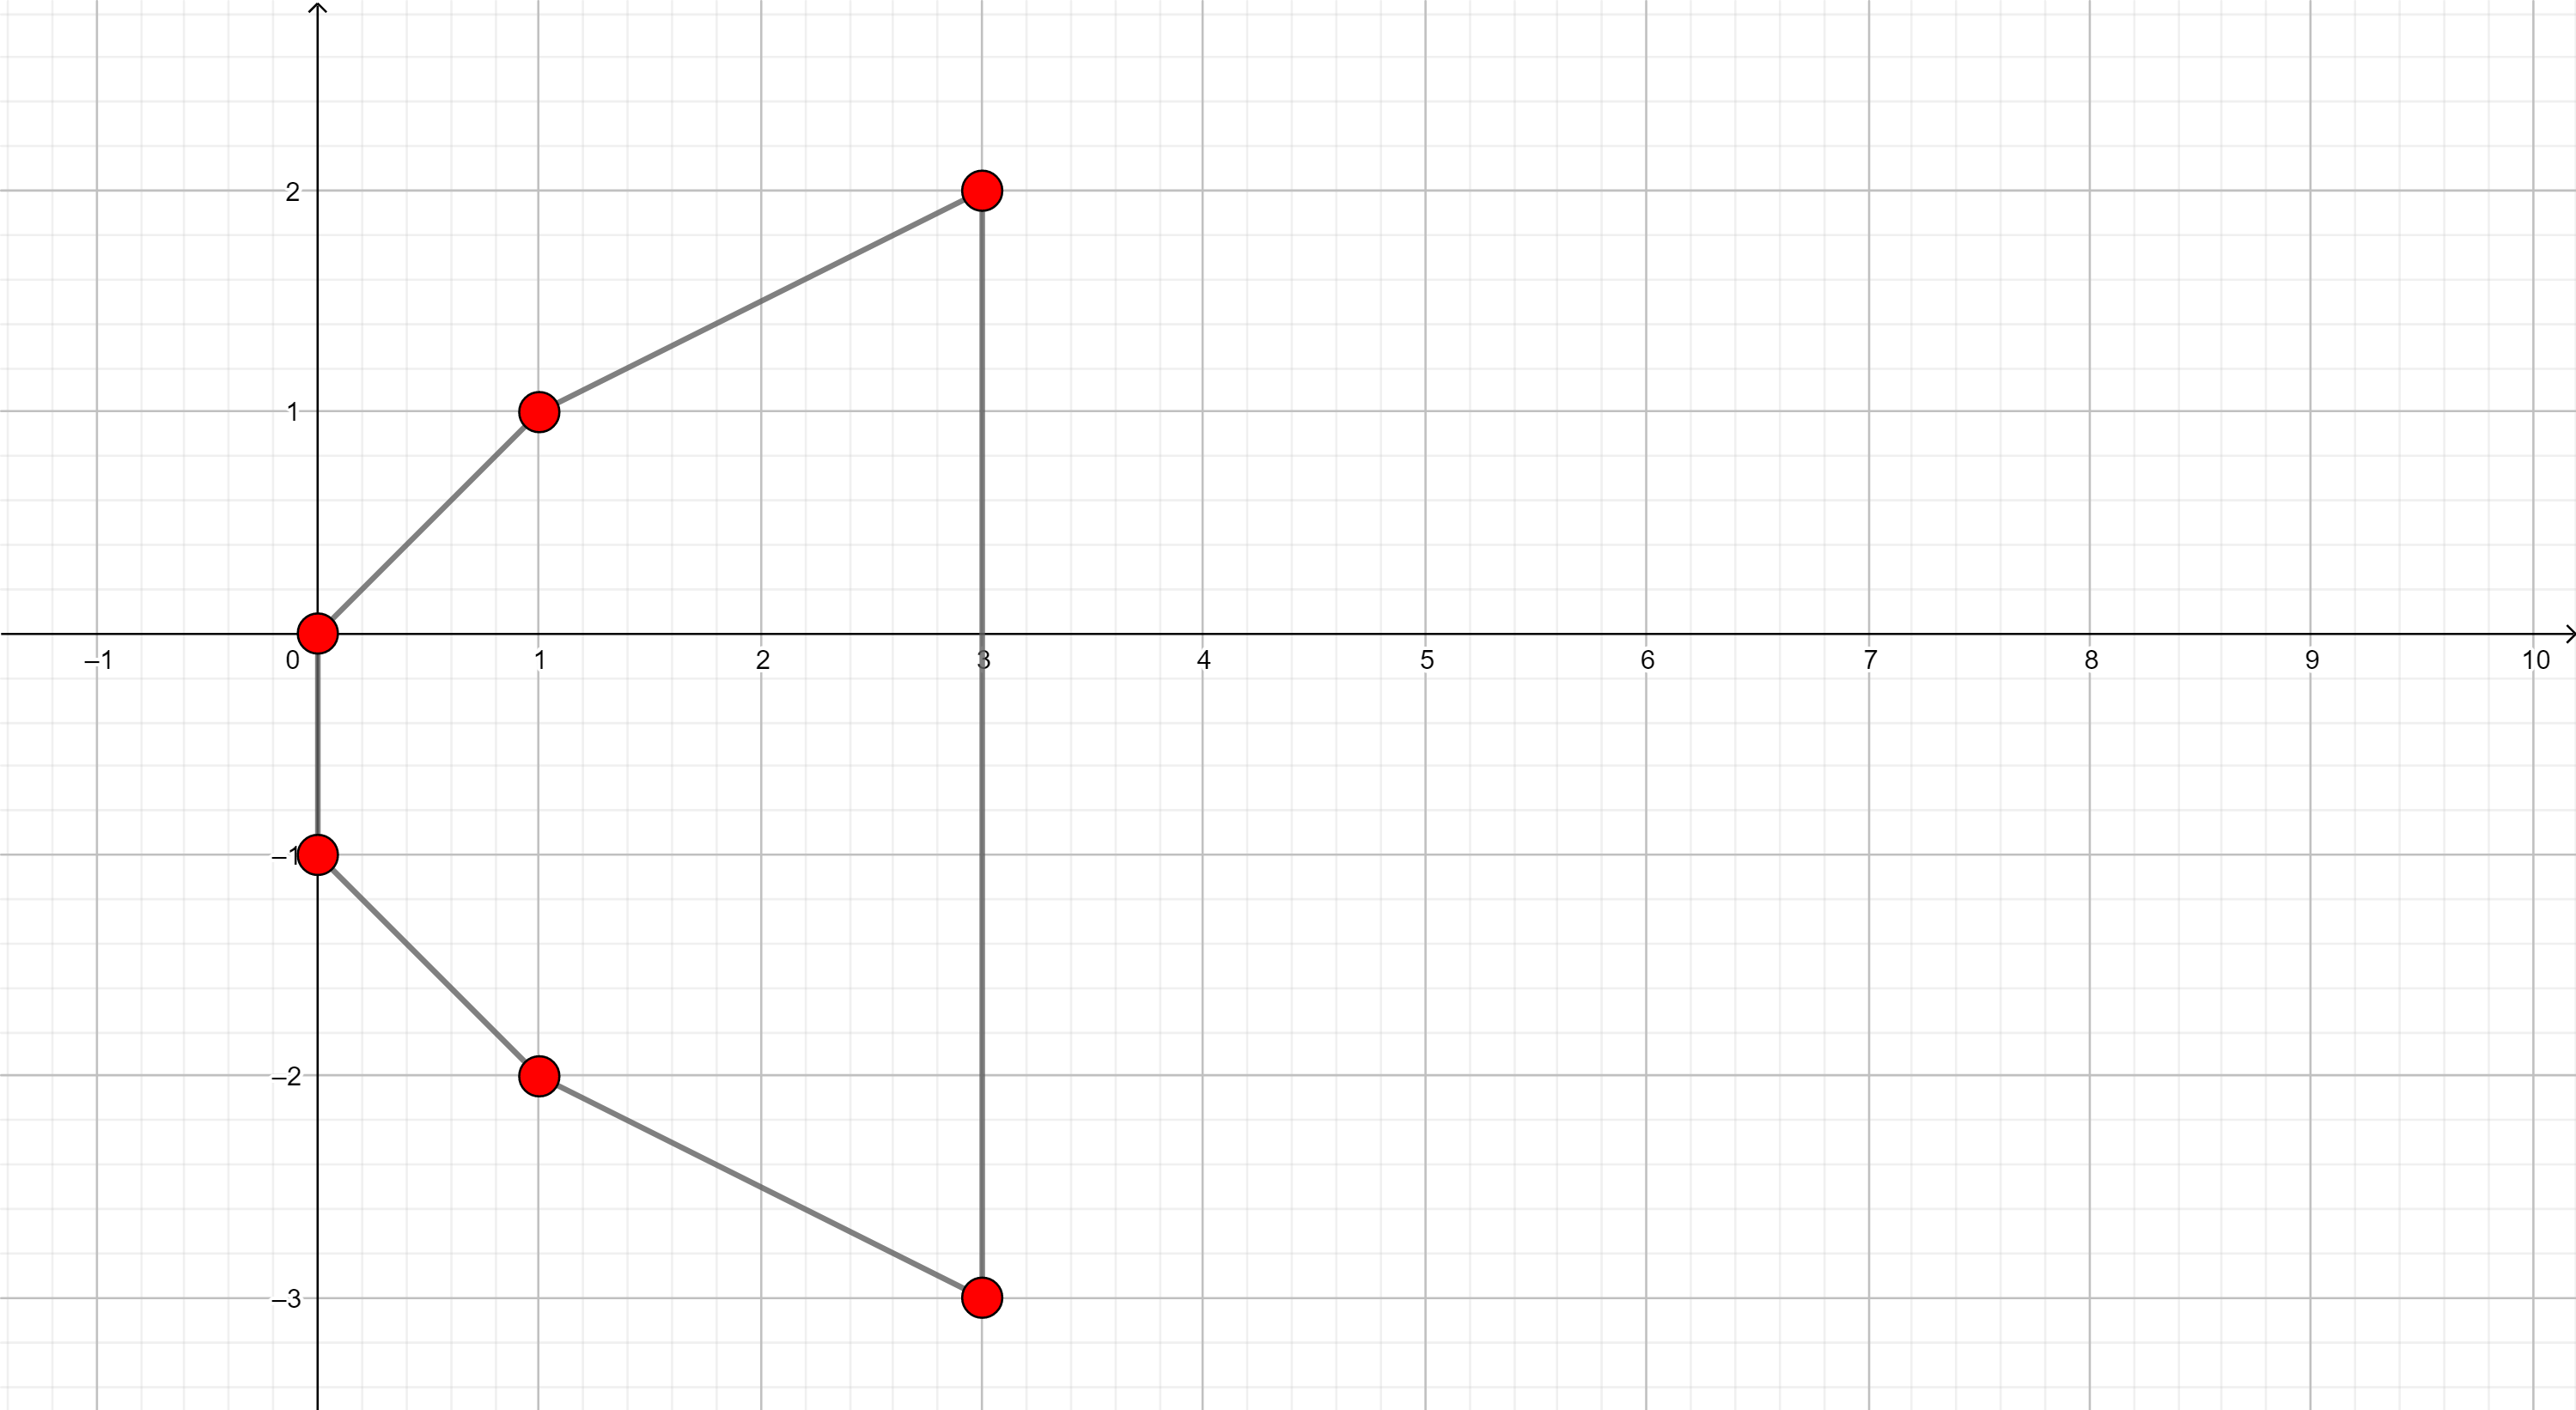
\includegraphics[scale=0.5]{poly3.png}}
\fbox{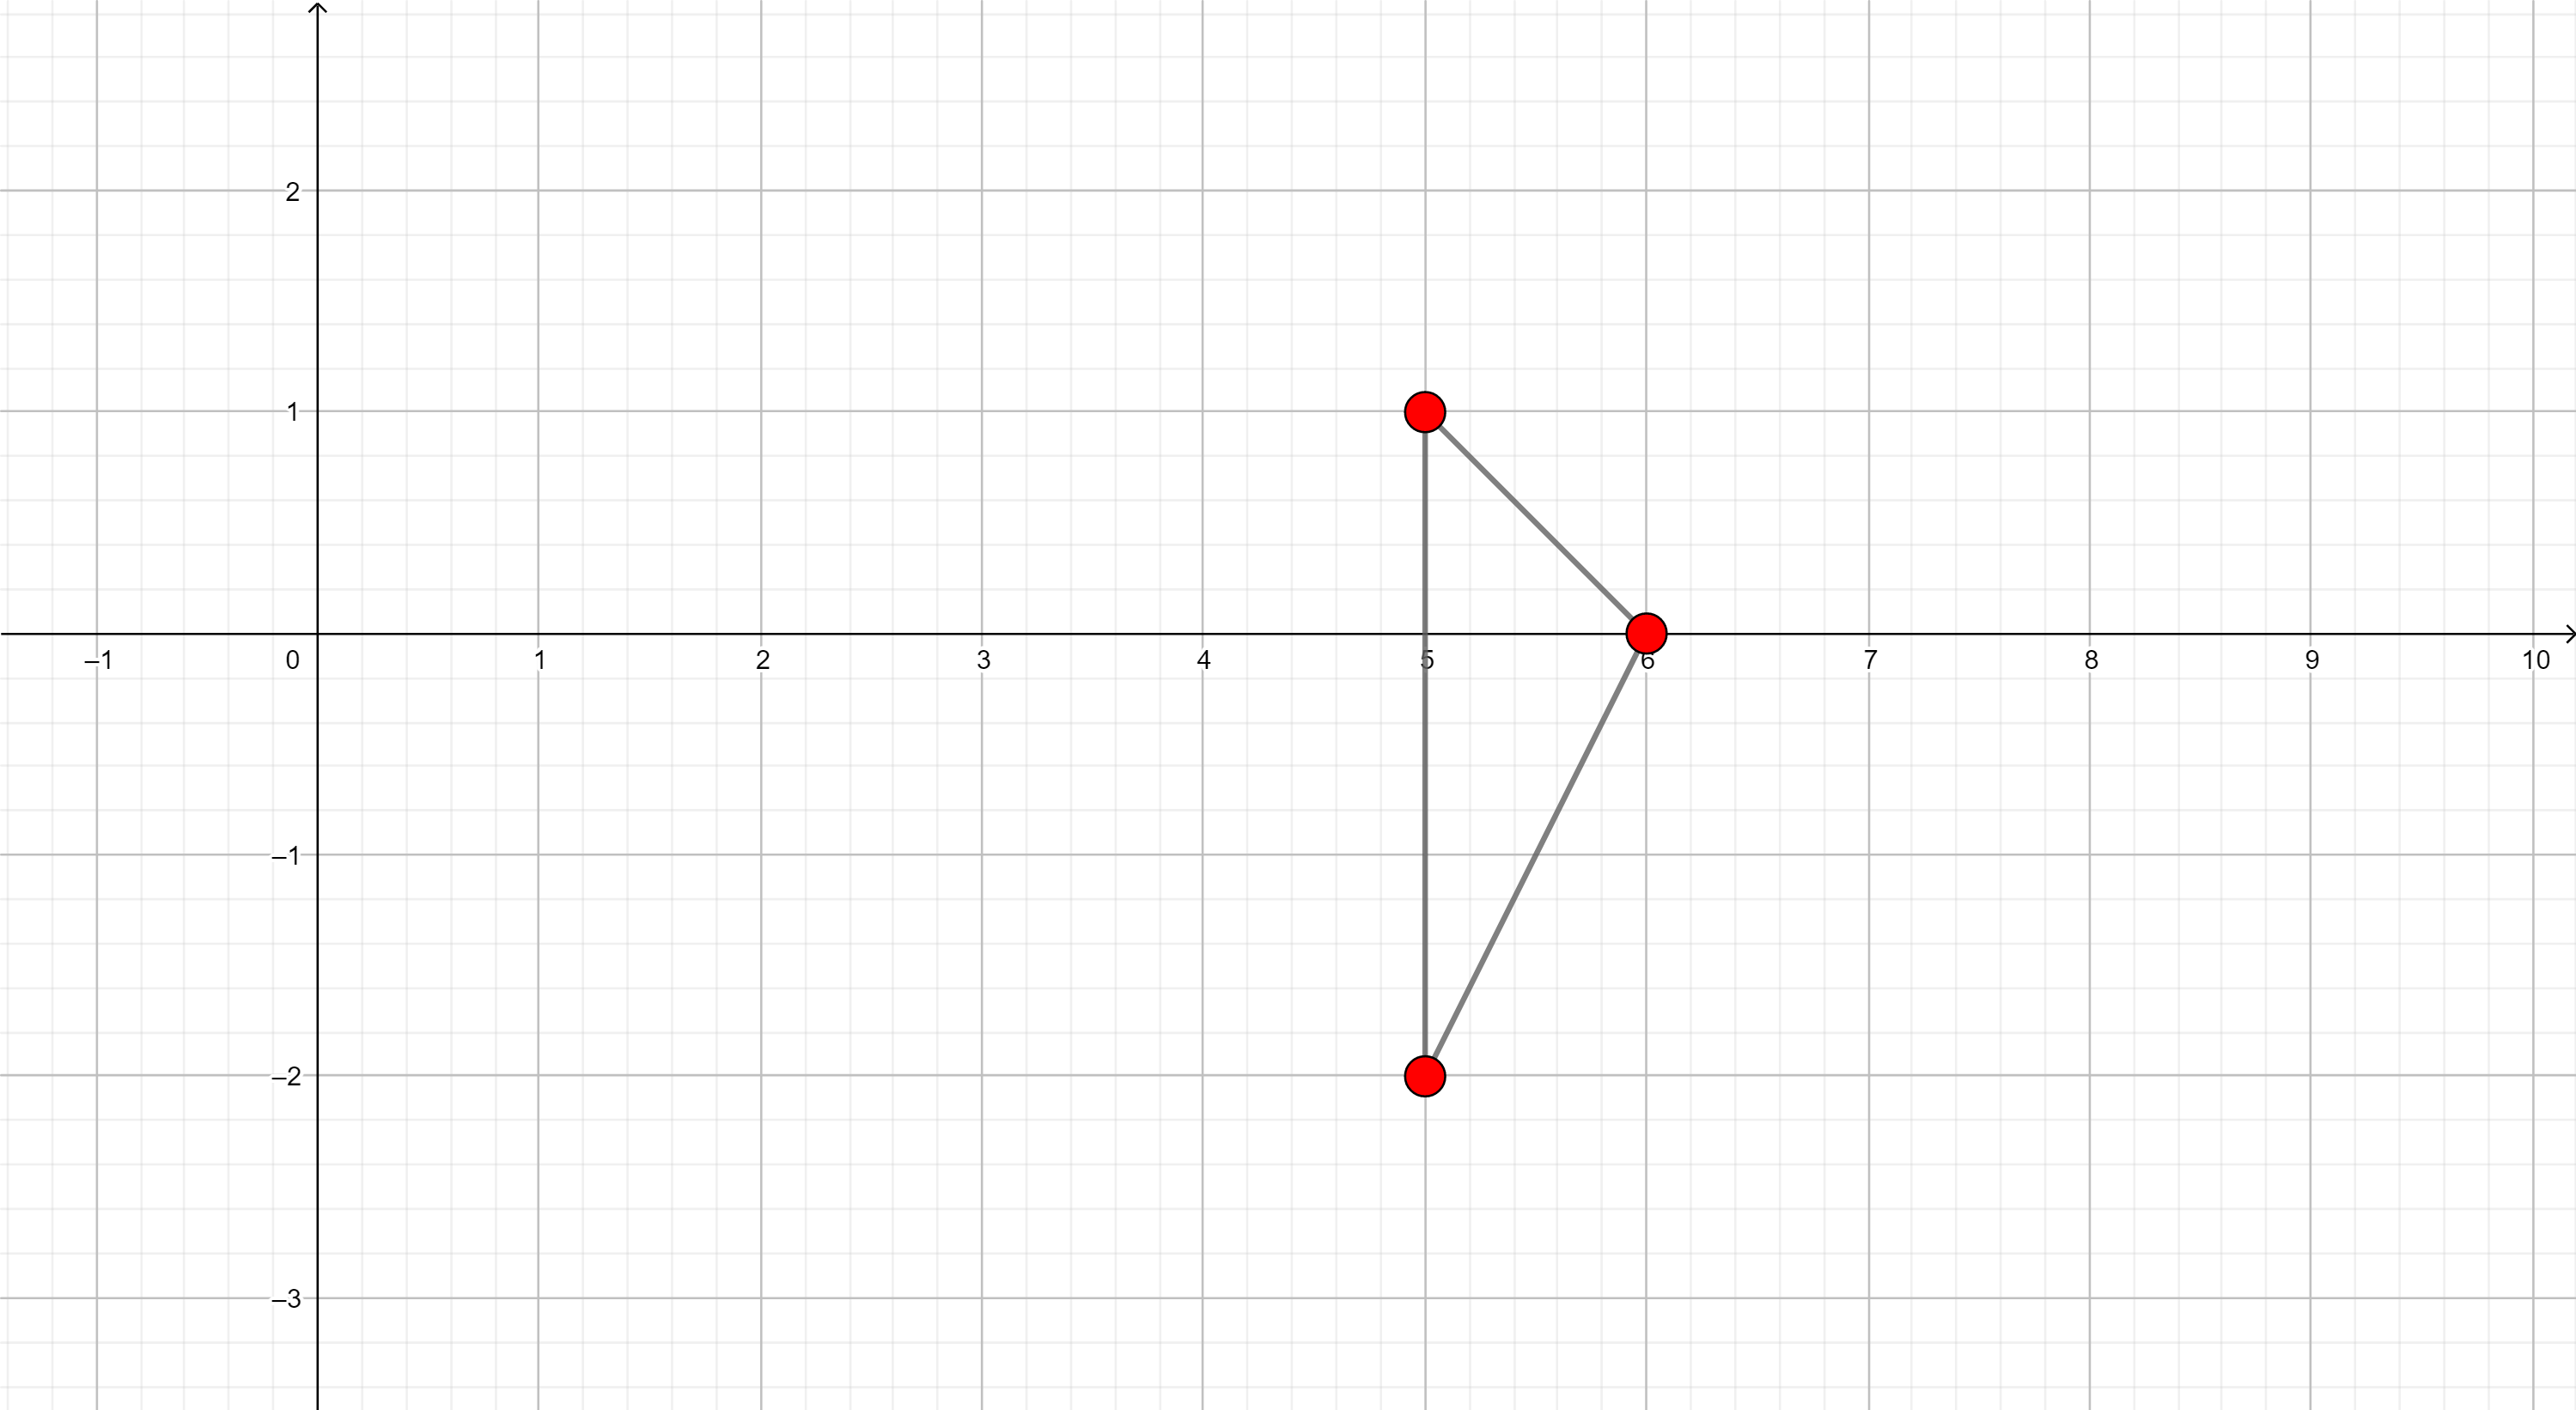
\includegraphics[scale=0.5]{poly4.png}}   
\end{center}
Pada hari ke-5 dan ke-6 Arvy melepas seluruh paku di dindingnya, sehingga luas poligon yang terbentuk nol (lihat catatan pada deskripsi).
\end{document}